\documentclass[../hw4]{subfiles}

\begin{document}

\begin{enumerate}[label= (\alph*)]
    \item Prove the triangle identity in $\mathbb{C}$, \[|z+\omega|\leq|z|+|\omega|.\]
    
    \begin{proposition}[*]
        The square of the norm of a number is the product of a number and its conjugate, \[{|z|}^2=z\bar{z}.\]
    \end{proposition}

    \begin{proof}[Proof of (*).]
        Let $z=\alpha + \beta i$.

        So, $|z|=\sqrt{\alpha^2+\beta^2}$ and ${|z|}^2=\alpha^2+\beta^2$.

        Then, $z\bar{z}=(\alpha+\beta i)(\alpha - \beta i)=\alpha^2-\beta^2 i^2 = \alpha^2 + \beta^2$.

        It is now clear that ${|z|}^2=z\bar{z}$.
    \end{proof}

    \begin{proposition}[**]
        The conjugate of a sum of two numbers is equal to the sum of their conjugates, \[\overline{z+\omega}=\bar{z}+\bar{\omega}.\]
    \end{proposition}

    \begin{proposition}[***]
        The conjugate of a product of two numbers is equal to the product of their conjugates, \[\overline{z\omega}=\bar{z}\bar{\omega}.\]
    \end{proposition}

    \begin{proposition}[****]
        The sum of a number and its conjugate is equal to twice the real part of the number, \[z+\bar{z}=2\,\text{Re}[z].\]
    \end{proposition}

    \begin{proof}[Proof of (****).]
        Let $z=\alpha+\beta i$. Then $\text{Re}[z]=\alpha$.
        
        With $\bar{z}=\alpha-\beta i$, $z+\bar{z}=\alpha+\beta i + \alpha - \beta i=2\alpha=2\,\text{Re}[z]$.
    \end{proof}

    \begin{proposition}[*****]
        The norm of a number is equal to the norm of its conjugate, \[|z|=|\bar{z}|.\]
    \end{proposition}

    \begin{proposition}[******]
        The norm of a product of two numbers is equal to the product of their norms, \[|z\omega|=|z||\omega|.\]
    \end{proposition}

    \begin{proof}[Proof of (******).]
        Let $z=a+bi$ and $\omega=x+yi$.

        Then,
        \begin{align*}
            z\omega&=ax+ayi+bxi+byi^2\\
            &=(ax-by)+(ay+bx)i. \\
        \end{align*}

        So,
        \begin{align*}
            |z\omega|&=\sqrt{{ax-by}^2+{ay+bx}^2} \\
            &= \sqrt{a^2x^2-2abxy+b^2y^2+a^2y^2+2abxy+b^2x^2}\\
            &= \sqrt{a^2x^2+b^2y^2+a^2y^2+b^2x^2} \\
            &= \sqrt{(a^2+b^2)(x^2+y^2)}. \\
        \end{align*}

        With $|z|=\sqrt{a^2+b^2}$ and $|\omega|=\sqrt{x^2+y^2}$, then
        \[|z||\omega|=\sqrt{(a^2+b^2)(x^2+y^2)}.\]
        
        So, the proposition holds.
    \end{proof}

    \begin{lemma}
        \[z\bar{\omega}+\bar{z}\omega\leq 2|z||\omega|.\]
    \end{lemma}

    \begin{proof}[Proof of Lemma.]
        Since $\overline{z\bar{\omega}}=\bar{z}\omega$ by (***), then $z\bar{\omega} + \bar{z}\omega = 2\,\text{Re}[z\bar{\omega}]$ by (****).

        Since $\text{Re}[z]\leq z$, then $2\,\text{Re}[z\bar{\omega}]\leq2|z\bar{\omega}|$.

        But, $2|z\bar{\omega}|=2|z||\omega|$ by (*****) and (******).

        So, $z\bar{\omega}+\bar{z}\omega\leq 2|z||\omega|$ and the Lemma holds.
    \end{proof}

    \begin{proof}[Proof of statement.]
        We begin with
        \begin{align*}
            {|z+\omega|}^2&=(z+\omega)(\bar{z}+\bar{\omega}) \quad\text{by (*) and (**)} \\
            &= z\bar{z}+z\bar{\omega}+\bar{z}\omega+\omega\bar{\omega}\\
            &= {|z|}^2+z\bar{\omega}+\bar{z}\omega+{|\omega|}^2 \quad\text{by (*)}\\
            &\leq{|z|}^2+2|z||\omega|+{|\omega|}^2 \quad\text{by the Lemma} \\
            &={(|z|+|\omega|)}^2. \\
        \end{align*}

        Since \[{|z+\omega|}^2\leq{(|z|+|\omega|)}^2,\]

        then, \[|z+\omega|\leq|z|+|\omega|\] holds as well.
    \end{proof}

    \begin{figure*}[ht]
    \centering
    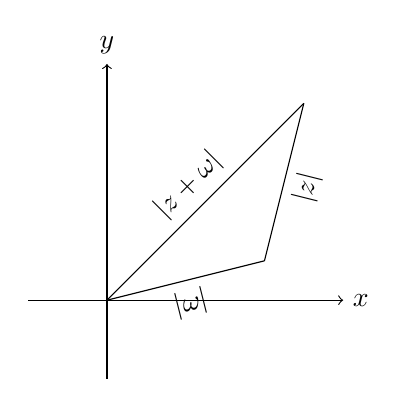
\begin{tikzpicture}
        \draw[->] (0,-1) -- (0,3) node[above] {$y$};
        \draw[->] (-1,0) -- (3,0) node[right] {$x$};
    
        \draw (0,0) -- (2,0.5) node[midway, below,sloped] {$|\omega|$};
        \draw (2,0.5) -- (2.5,2.5) node[midway, below, sloped] {$|z|$};
        \draw (0,0) -- (2.5,2.5) node[midway, above, sloped] {$|z+\omega|$};
    \end{tikzpicture}
    \caption{Proof of triangle inequality in the complex plane.}
    \end{figure*}

    % \begin{figure*}[ht]
    % \centering
    % \begin{tikzpicture}
    %     % Draw the coordinate grid
    %     \draw[thin,gray!40] (-2,-2) grid (4,4);
    %     \draw[thick,->] (-2,0)--(4,0) node[right]{$\Re$}; % x-axis
    %     \draw[thick,->] (0,-2)--(0,4) node[above]{$\Im$}; % y-axis
      
    %     % Define complex numbers z and w
    %     \pgfmathsetmacro{\zx}{3} % Real part of z
    %     \pgfmathsetmacro{\zy}{2} % Imaginary part of z
    %     \pgfmathsetmacro{\wx}{1} % Real part of w
    %     \pgfmathsetmacro{\wy}{1} % Imaginary part of w
      
    %     % Draw vectors
    %     \draw[->, thick, blue] (0,0) -- (\zx,\zy) node[midway,above] {$z$};
    %     \draw[->, thick, red] (\zx,\zy) -- (\zx+\wx,\zy+\wy) node[midway,above] {$w$};
    %     \draw[->, thick, green] (0,0) -- (\zx+\wx,\zy+\wy) node[midway,below] {$z+w$};
      
    %     % Draw triangle
    %     \draw[dashed] (\zx,\zy) -- (\zx,\zy+\wy);
    %     \draw[dashed] (\zx,\zy+\wy) -- (\zx+\wx,\zy+\wy);
    % \end{tikzpicture}
    % \end{figure*}

    \item Prove that, \[{|z+\omega|}^2+{|z-\omega|}^2=2\left( {|z|}^2+{|\omega|}^2 \right).\]
    
    \begin{proof}
        We proceed with the propositions (*) and (**) above,
        \begin{align*}
            {|z+\omega|}^2+{|z-\omega|}^2 &= (z+\omega)(\bar{z}+\bar{\omega})+(z-\omega)(\bar{z}-\bar{\omega}) \\
            &= z\bar{z}+\bar{z}\omega+z\bar{\omega}+\omega\bar{\omega}+z\bar{z}-\bar{z}\omega-\bar{\omega}z+\omega\bar{\omega} \\
            &= 2z\bar{z}+2\omega\bar{\omega} \\
            &= 2\left( {|z|}^2+{|\omega|}^2 \right). \\
        \end{align*}
    \end{proof}
\end{enumerate}

\end{document}